\actTitle{4.5 - Graphs of Sine and Cosine Functions}

\videoLink{Section 4.5 day 1}{https://www.youtube.com/playlist?list=PLYHZK3b8UFw0U_iMosD8HZraus76s5k2i}
% \videoLink{Section 4.5 day 2}{https://www.youtube.com/playlist?list=PLYHZK3b8UFw0U_iMosD8HZraus76s5k2i}

\noindent \textbf{Topics:}  graphs of $a\sin(bx+c)$ and $a\cos(bx+c)$, period, amplitude, and phase shift\\

\noindent \textbf{Student Learning Outcomes:}
\begin{enumerate}
\item Students will be able to graph $a\sin(bx+c)$ and $a\cos(bx+c)$.
\item Students will be able to determine a sine and cosine wave given a written description.
\item Students will be able to determine the formula for a sine or cosine wave given the graph of the function.
\end{enumerate}

\hrule 

\bigskip

\subsection{Graph $y=\sin(x)$ and $y=\cos(x)$} ~


\noindent
  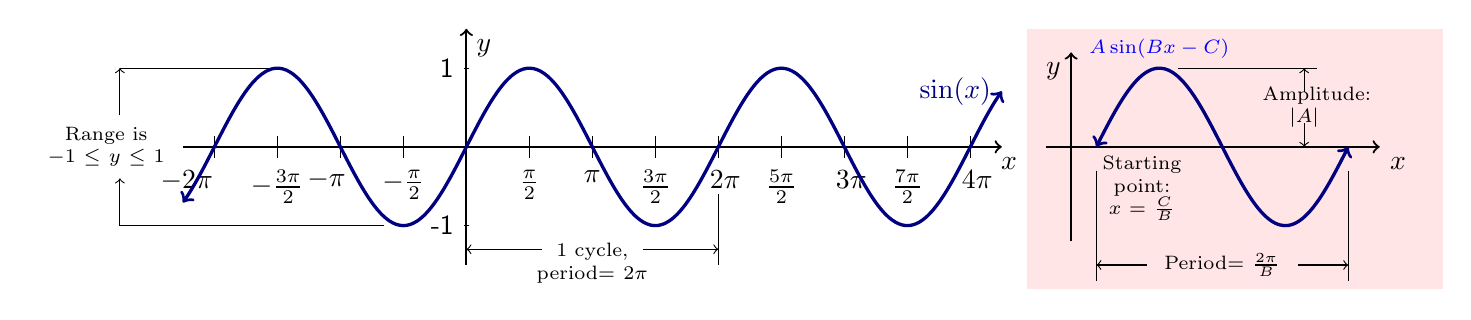
\begin{tikzpicture}[y=1.0cm, x=0.8cm,font=\sffamily]
    \begin{scope}
      %% ticks
      % \draw[step = 1.0, gray,dashed] (-3,-1.2) grid (3,1.2);
      %% axis
      \draw[thick,->] (-4.5,0) -- coordinate (x axis mid) (8.5,0)
           node[anchor = north west,xshift=-4] {$x$};
      \draw[thick,->] (0,-1.5) -- coordinate (y axis mid) (0,1.5)
           node[anchor = north west] {$y$};
      \foreach \y in {-1,1} {
        \draw (1pt, \y) -- (-1pt, \y) node[anchor=east] {\y};
      }
      \foreach \x in {-4,-3,...,8} {
        \draw(\x,4pt) -- (\x,-4pt);
      }

      \node[yshift=-5,xshift=0,anchor=north] at (1,0) {$\frac{\pi}{2}$};
      \node[yshift=-5,xshift=0,anchor=north] at (2,0) {$\pi$};
      \foreach \x in {3,5,7} {
        \node[yshift=-5,xshift=0,anchor=north] at (\x,0) {$\frac{\x\pi}{2}$};
      }
      \foreach \x in {2,3,4} {
        \node[yshift=-5,xshift=2.5,anchor=north] at (2*\x,0) {$\x\pi$};
      }

      \node[yshift=-5,xshift=0,anchor=north] at (-1,0)  {$-\frac{\pi}{2}$};
      \node[yshift=-5,xshift=-5,anchor=north] at (-2,0) {$-\pi$};
      \node[yshift=-5,xshift=0,anchor=north] at (-3,0)  {$-\frac{3\pi}{2}$};
      \node[yshift=-5,xshift=-10,anchor=north] at (-4,0) {$-2\pi$};

      \draw[black] (4,-0.6) -- (4,-1.5);
      \draw[black,<-] (0,-1.3) -- (1.2,-1.3);
      \draw[black,->] (2.8,-1.3) -- (4,-1.3);
      \node[black,align=center,text width=5em,font=\scriptsize,yshift=-5] at (2,-1.3)
           {1 cycle, period$=2\pi$};

      \draw[black] (-1.3,-1) -- (-5.5,-1);
      \draw[black] (-3.1, 1) -- (-5.5, 1);
      \draw[black,->] (-5.5, 0.4) -- (-5.5,1);
      \draw[black,<-] (-5.5,-0.4) -- (-5.5,-1);
      \node[black,align=center,text width=5em,font=\scriptsize,xshift=-5] at (-5.5,0)
         {Range is $-1\leq y \leq 1$};

      \begin{scope}
        %% \clip(-4,-1) rectangle (8,5);
        \draw[scale=1.0,domain=-4.5:8.5,smooth,variable=\x,very thick,blue!50!black,samples=120,<->]
           plot ({\x},{sin(deg(0.5*pi*\x))}) node[anchor=east] {$\sin(x)$};
      \end{scope}
    \end{scope}

    \begin{scope}[shift={(10,0)},scale=1.0]
      \fill [red!10!white] (-1.1,-1.8) rectangle (5.5,1.5);
      \draw[thick,->] (-0.8,0) -- coordinate (x axis mid) (4.5,0)
           node[anchor = north west] {$x$};
      \draw[thick,->] (-0.4,-1.2) -- coordinate (y axis mid) (-0.4,1.2)
           node[anchor = north east] {$y$};
      \begin{scope}
        %% \clip(-4,-1) rectangle (8,5);
        \draw[scale=1.0,domain=0:4,smooth,variable=\x,very thick,blue!50!black,samples=60,<->]
           plot ({\x},{sin(deg(0.5*pi*\x))});
      \end{scope}
      \node[anchor=south,font=\scriptsize,blue] at (1,1) {$A\sin(Bx-C)$};   
      \draw[black] (0,-0.3) -- (0,-1.7);
      \draw[black] (4,-0.3) -- (4,-1.7);
      \draw[black,<-] (0,-1.5) -- (0.8,-1.5);
      \draw[black,->] (3.2,-1.5) -- (4,-1.5);
      \node[black,align=center,text width=5em,font=\scriptsize,yshift=0] at (2,-1.5)
           {Period$=\frac{2\pi}{B}$};
      \node[black,align=center,text width=3em,font=\scriptsize,xshift=-2,anchor=north west] at (0,0)
           {Starting point: $x=\frac{C}{B}$};

      \draw[black] (1.3,1) -- (3.5,1);
      \draw[black,->] (3.3, 0.7) -- (3.3,1);
      \draw[black,<-] (3.3, 0.0) -- (3.3,0.3);
      \node[black,align=center,text width=3em,font=\scriptsize,xshift=0] at (3.3,0.5)
          {Amplitude: $|A|$};
    \end{scope}
  \end{tikzpicture}

\noindent
  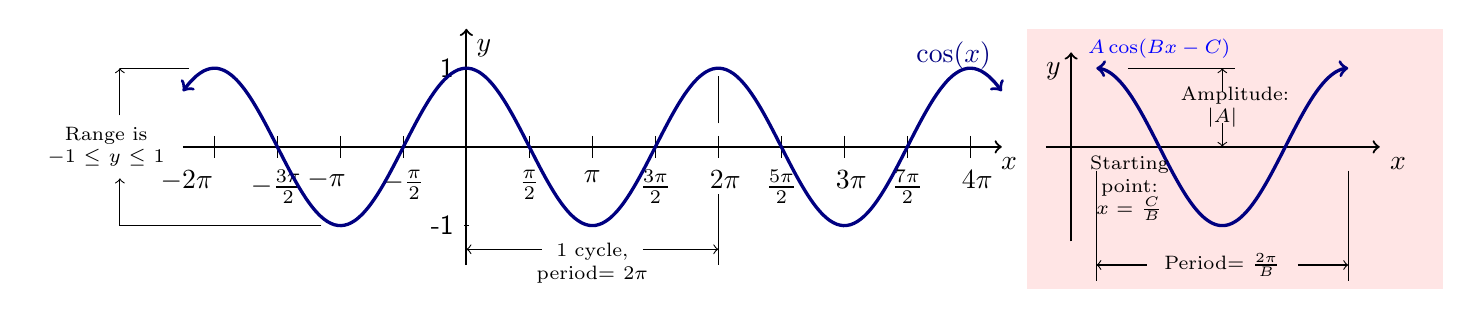
\begin{tikzpicture}[y=1.0cm, x=0.8cm,font=\sffamily]
    \begin{scope}
      %% ticks
      % \draw[step = 1.0, gray,dashed] (-3,-1.2) grid (3,1.2);
      %% axis
      \draw[thick,->] (-4.5,0) -- coordinate (x axis mid) (8.5,0)
           node[anchor = north west,xshift=-4] {$x$};
      \draw[thick,->] (0,-1.5) -- coordinate (y axis mid) (0,1.5)
           node[anchor = north west] {$y$};
      \foreach \y in {-1,1} {
        \draw (1pt, \y) -- (-1pt, \y) node[anchor=east] {\y};
      }
      \foreach \x in {-4,-3,...,8} {
        \draw(\x,4pt) -- (\x,-4pt);
      }

      \node[yshift=-5,xshift=0,anchor=north] at (1,0) {$\frac{\pi}{2}$};
      \node[yshift=-5,xshift=0,anchor=north] at (2,0) {$\pi$};
      \foreach \x in {3,5,7} {
        \node[yshift=-5,xshift=0,anchor=north] at (\x,0) {$\frac{\x\pi}{2}$};
      }
      \foreach \x in {2,3,4} {
        \node[yshift=-5,xshift=2.5,anchor=north] at (2*\x,0) {$\x\pi$};
      }

      \node[yshift=-5,xshift=0,anchor=north] at (-1,0)  {$-\frac{\pi}{2}$};
      \node[yshift=-5,xshift=-5,anchor=north] at (-2,0) {$-\pi$};
      \node[yshift=-5,xshift=0,anchor=north] at (-3,0)  {$-\frac{3\pi}{2}$};
      \node[yshift=-5,xshift=-10,anchor=north] at (-4,0) {$-2\pi$};

      \draw[black] (4,-0.6) -- (4,-1.5);
      \draw[black] (4,0.3) -- (4,0.9);
      \draw[black,<-] (0,-1.3) -- (1.2,-1.3);
      \draw[black,->] (2.8,-1.3) -- (4,-1.3);
      \node[black,align=center,text width=5em,font=\scriptsize,yshift=-5] at (2,-1.3)
           {1 cycle, period$=2\pi$};

      \draw[black] (-2.3,-1) -- (-5.5,-1);
      \draw[black] (-4.4, 1) -- (-5.5, 1);
      \draw[black,->] (-5.5, 0.4) -- (-5.5,1);
      \draw[black,<-] (-5.5,-0.4) -- (-5.5,-1);
      \node[black,align=center,text width=5em,font=\scriptsize,xshift=-5] at (-5.5,0)
         {Range is $-1\leq y \leq 1$};

      \begin{scope}
        %% \clip(-4,-1) rectangle (8,5);
        \draw[scale=1.0,domain=-4.5:8.5,smooth,variable=\x,very thick,blue!50!black,samples=120,<->]
           plot ({\x},{cos(deg(0.5*pi*\x))}) node[anchor=south east,yshift=4] {$\cos(x)$};
      \end{scope}
    \end{scope}

    \begin{scope}[shift={(10,0)},scale=1.0]
      \fill [red!10!white] (-1.1,-1.8) rectangle (5.5,1.5);
      \draw[thick,->] (-0.8,0) -- coordinate (x axis mid) (4.5,0)
           node[anchor = north west] {$x$};
      \draw[thick,->] (-0.4,-1.2) -- coordinate (y axis mid) (-0.4,1.2)
           node[anchor = north east] {$y$};
      \begin{scope}
        %% \clip(-4,-1) rectangle (8,5);
        \draw[scale=1.0,domain=0:4,smooth,variable=\x,very thick,blue!50!black,samples=60,<->]
           plot ({\x},{cos(deg(0.5*pi*\x))});
      \end{scope}
      \node[anchor=south,font=\scriptsize,blue] at (1,1) {$A\cos(Bx-C)$};   
      \draw[black] (0,-0.3) -- (0,-1.7);
      \draw[black] (4,-0.3) -- (4,-1.7);
      \draw[black,<-] (0,-1.5) -- (0.8,-1.5);
      \draw[black,->] (3.2,-1.5) -- (4,-1.5);
      \node[black,align=center,text width=5em,font=\scriptsize,yshift=0] at (2,-1.5)
           {Period$=\frac{2\pi}{B}$};
      \node[black,align=center,text width=3em,font=\scriptsize,xshift=-2,anchor=north west] at (-0.2,0)
           {Starting point: $x=\frac{C}{B}$};

      \draw[black] (0.5,1) -- (2.2,1);
      \draw[black,->] (2.0, 0.7) -- (2.0,1);
      \draw[black,<-] (2.0, 0.0) -- (2.0,0.3);
      \node[black,align=center,text width=3em,font=\scriptsize,xshift=0] at (2.0,0.5)
          {Amplitude: $|A|$};
    \end{scope}
  \end{tikzpicture}


  \noindent \underline{Recall} The period of the sine graph is $2\pi$;
  the period of the cosine graph is also $2\pi$.


\begin{enumerate}
\vspace{-.1in}
\item \begin{enumerate} \item Explain how to obtain the graph of $f(x)=-3\sin(x)$ from the graph of $y=\sin(x)$.\\[.5in]
\item Sketch the graph of the function $f(x)= -3\sin(x)$. \\
\scalebox{.8}{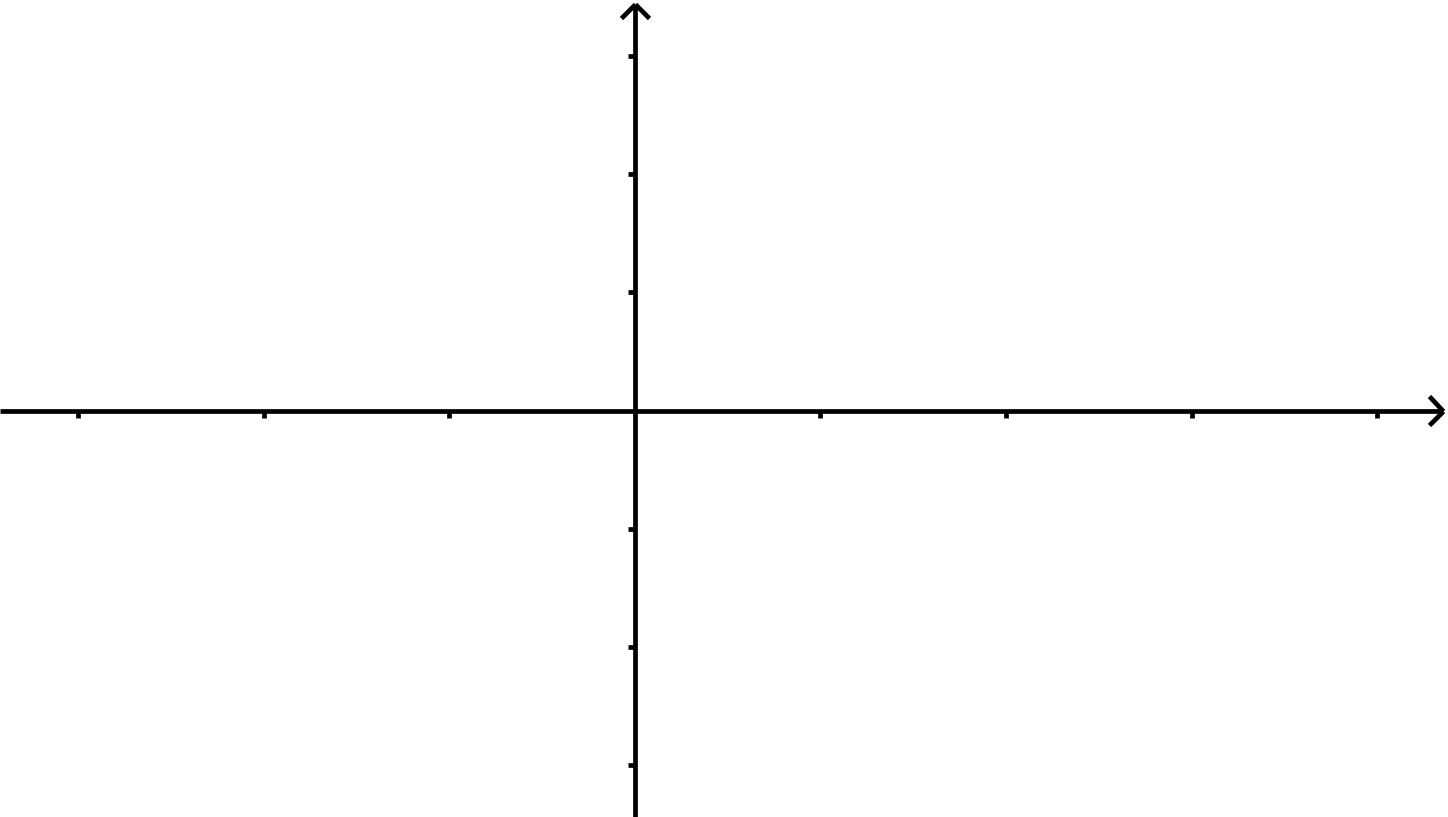
\includegraphics[scale=1.5]{gentrig1}}\\
\item Determine the period and amplitude of the function $f(x)= -3\sin(x)$. \\[1in]
\end{enumerate}



\hspace{-.3in} \begin{tabular}{| l | }
\hline 
For a function $y=A\sin(Bx+C)$ or $y=A \cos(Bx+C)$, assuming that $A$ and $B$ are both not zero, \\

$\star$ The \emph{amplitude} is $|A|$.\\
$\star$ The \emph{period} is $2\pi/|B|$.   \\
$\star$ The \emph{phase shift} is $-C/B$. A negative phase shift is a shift to the left; a positive phase shift\\ is a shift to the right. You can get it from graph transformations if you do the horizontal shift \emph{last}.% \\
%$\star$ To find an interval containing exactly one cycle, solve the equations $0=bx+c$ and $2\pi = bx+c$. 
\\ \hline
\end{tabular}

\vfill
\textbf{How to Graph Sine and Cosine Functions}
\begin{enumerate}
\item Find amplitude, period, and phase shift.
\item Determine the interval of one period on the $x$-axis. (Set interval $0\leq Bx+C \leq 2\pi$ and solve.
\item Divide the interval into fourths to plot "key points".
\item Use rules for function transformation.
\end{enumerate}
\vfill


\newpage

\item \begin{enumerate} \item Explain how to obtain the graph of $f(x)=\sin(x+\pi/6)$ from the graph of $y=\sin(x)$. \\[.75in]

\item Determine the period, amplitude, and phase shift.\\[1.5in]

\item Find an interval containing exactly one cycle.\vfill

\item Sketch the graph of $f(x)=\sin(x+\pi/6)$. 
\end{enumerate} 

\scalebox{.8}{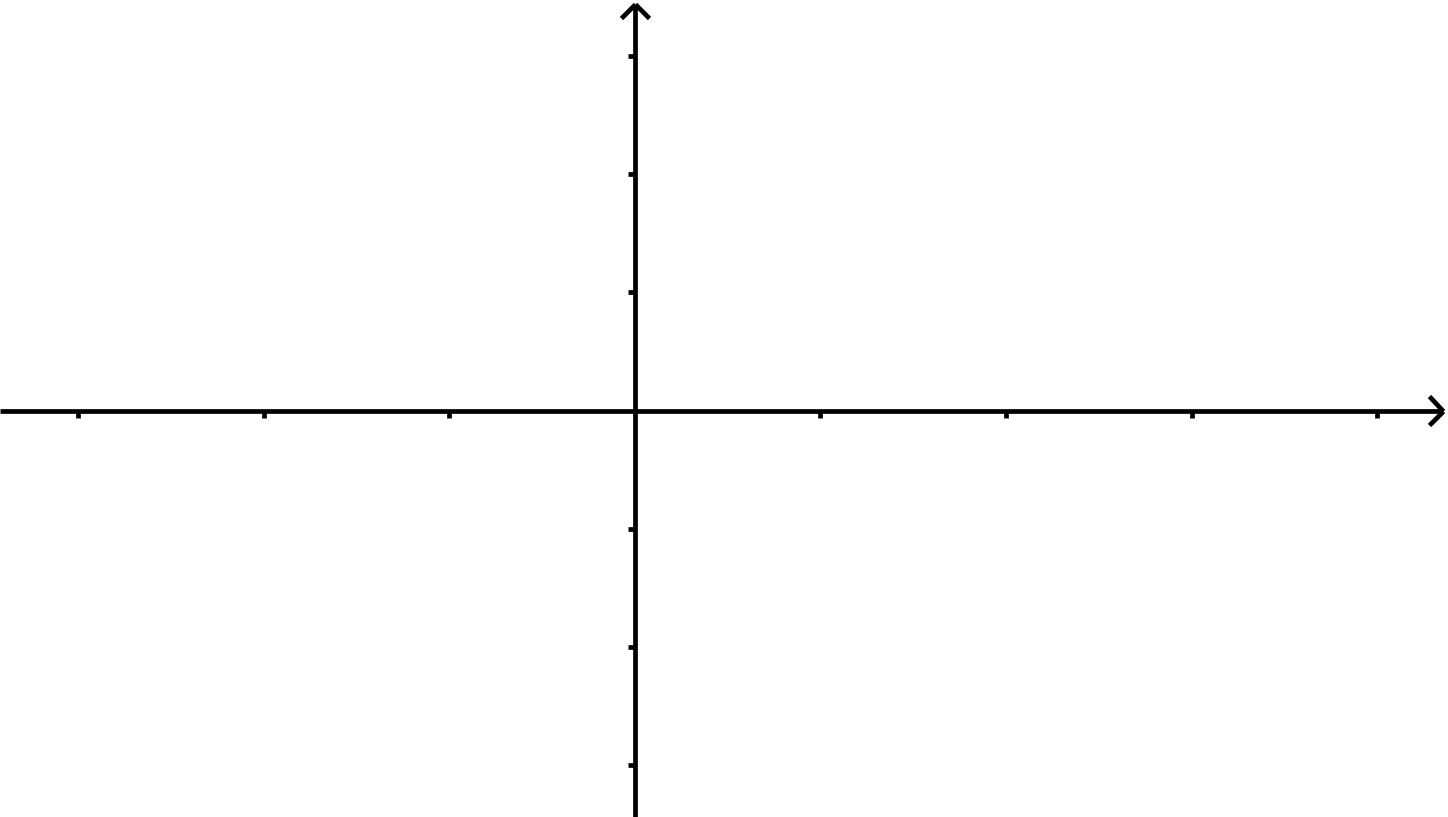
\includegraphics[scale=1.5]{gentrig1}}


\newpage

\item \begin{enumerate} \item Explain how to obtain the graph of $f(x)=3\cos(2x+\pi/2)$ from the graph of $y=\cos(x)$. \\[.75in]

\item Determine the period, amplitude, and phase shift.\\[1.5in]

\item Find an interval containing exactly one cycle.\vfill

\item Sketch the graph of $f(x)=3\cos(2x+\pi/2)$. 
\end{enumerate} 

\scalebox{.8}{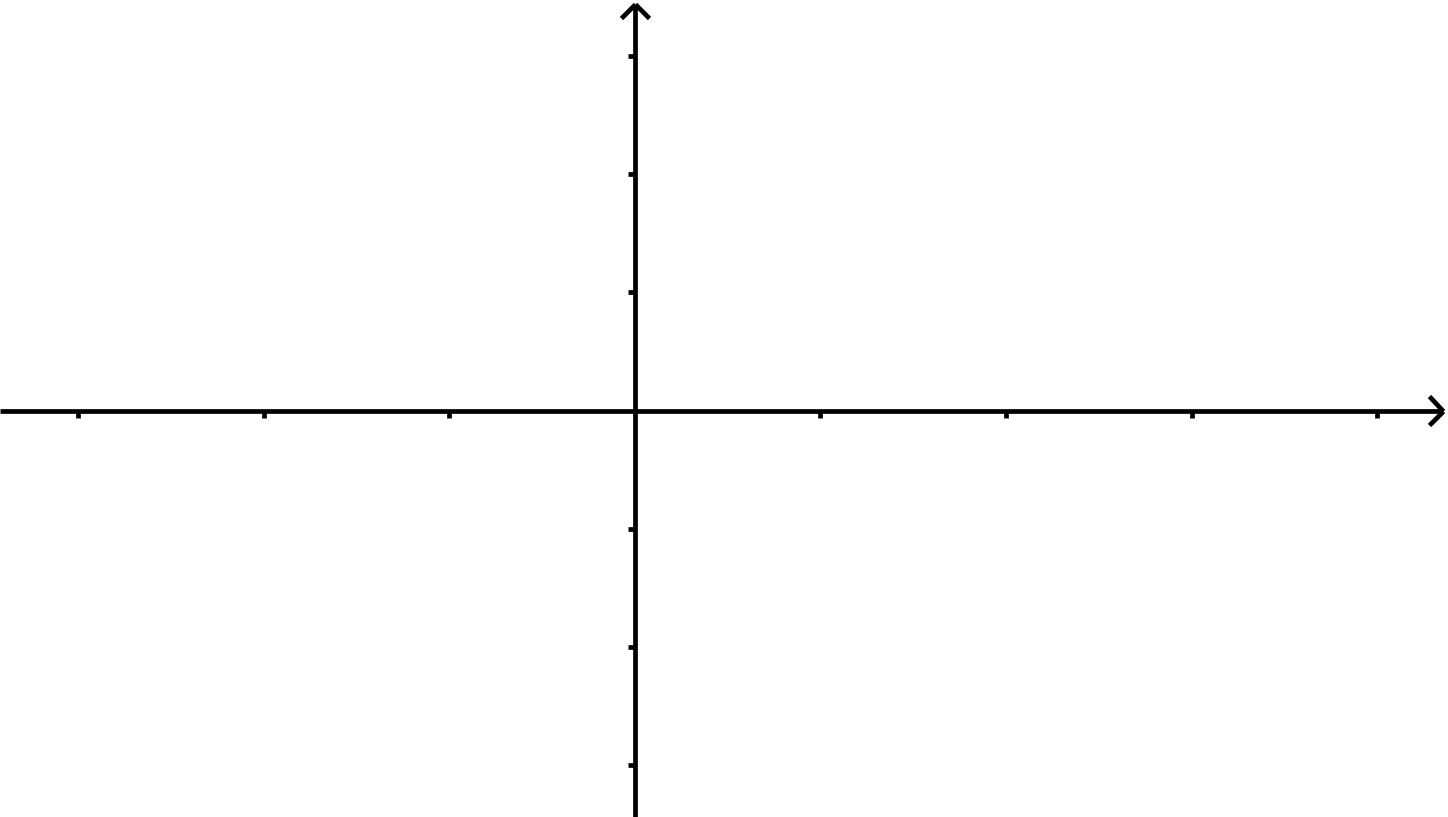
\includegraphics[scale=1.5]{gentrig1}}\\[.5in]



\newpage



\item Determine the period, amplitude, and phase shift of the function. \begin{enumerate}
\item $f(x)= -2 \sin(3x-7)$ \\[1in] 
%\item $g(x)= \cos\left(x+\dfrac{\pi}{7}\right)$ \\[.5in] 
\item $y = \cos\left(\dfrac{\pi x}{3}+\pi\right)$ \\[1in]
\end{enumerate}


\subsection{Determine a Formula for a Sine or Cosine Wave} ~

\item Express the equation for the sine wave shown below in the form
  $y=a\sin(bx+c)+d$. Then express the equation for the cosine wave
  shown below in the form $y=a\cos(bx+c)+d$.  In your equation, use
  $a>0$, $b>0$, and the least possible positive real number $c$.



 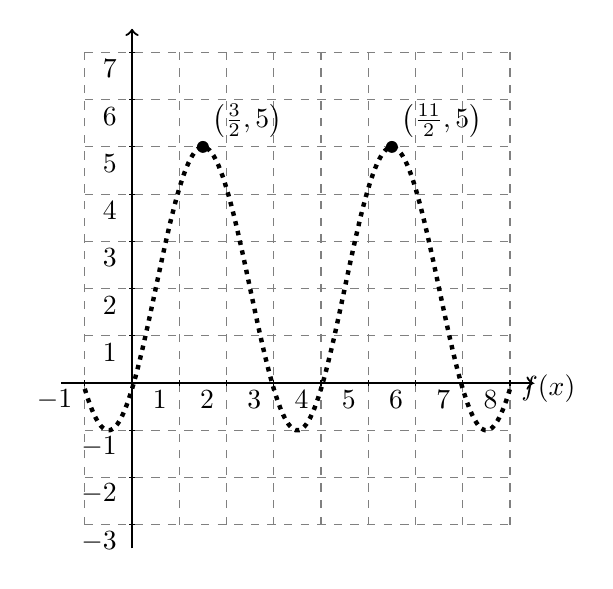
\begin{tikzpicture}[y=0.6cm, x=0.6cm,font=\sffamily]
    %% ticks
    \draw[step = 1, gray,dashed] (-1,-3) grid (8,7);
    %% axis
    \draw[thick,->] (-1.5,0) -- coordinate (x axis mid) (8.5,0) node[anchor = north west] {};
    \draw[thick,->] (0,-3.5) -- coordinate (y axis mid) (0,7.5) node[anchor = north east] {};
    \foreach \y in {-3,-2,-1,1,2,...,7} {
      \draw (1pt, \y) -- (-1pt, \y) node[yshift=-6,xshift=-1,anchor=east] {$\y$};
    }
    \foreach \x in {-1,1,2,...,8} {
      \draw (\x,1pt) -- (\x,-1pt) node[yshift=-5,xshift=-1,anchor=east] {$\x$};
    }

    \begin{scope}
      % \clip(-4,-1) rectangle (8,5);
%      \draw[scale=1.0,domain=-1:8,smooth,variable=\x,very thick,black,samples=120] 
%           plot ({\x},{2*cos(deg(pi*\x))-1}) node[anchor=west] {$f(x)$};
      \draw[scale=1.0,dotted,domain=-1:8,smooth,variable=\x,ultra thick,black,samples=120] 
          plot ({\x},{3*sin(deg(0.5*pi*\x-pi/4))+2}) node[anchor=west] {$f(x)$};
     \fill[black] (3/2,5) circle [radius=0.5ex] node[anchor=south west] {$\left(\frac{3}{2},5\right)$};
      \fill[black] (11/2,5) circle [radius=0.5ex] node[anchor=south west] {$\left(\frac{11}{2},5\right)$};
    \end{scope}

  \end{tikzpicture}



\vfill



%
%
%\newpage
%
%
%\subsection{Model Sinusoidal Behavior} ~
%
%
%\item The water level relative to the top of a boat dock varies with the tides.  One particular day, low tide occurs at midnight and the water level is 7ft below the dock.  The first high tide of the day occurs at approximately 6:00 AM, and the water level is 3ft below the dock.  The next low tide occurs at noon and the water level is again 7ft below the dock.\\
%
%Assuming that this pattern continues indefinitely and behaves like a cosine wave, write a function of the form $w(t)=A\cos(Bt+C)+D$.  The value $w(t)$ is the water level (in ft) relative to the top of the dock, $t$ hours after midnight.

\end{enumerate}
\vfill

\newpage
\noindent \textbf{Student Learning Outcomes Check}

\begin{enumerate}
\item Are you able to graph $a\sin(bx+c)$ and $a\cos(bx+c)$?
\item Can you determine a sine and cosine wave given a written description?
\item Can you determine the formula for a sine or cosine wave given the graph of the function?

\end{enumerate}

\noindent \textbf{If any of your answers were no, please ask about these topics in class.}

